\documentclass[a4paper, 12pt]{article}
\usepackage[T2A]{fontenc}
\usepackage[utf8]{inputenc}
\usepackage[english,russian]{babel}
\usepackage{amsmath, amsfonts, amssymb, amsthm, mathtools, misccorr, indentfirst, multirow}
\usepackage{wrapfig}
\usepackage{graphicx}
\usepackage{subfig}
\usepackage{adjustbox}
\usepackage{pgfplots}

\usepackage{geometry}
\geometry{top=20mm}
\geometry{bottom=20mm}
\geometry{left=20mm}
\geometry{right=20mm}
\newcommand{\angstrom}{\textup{\AA}}

\begin{document}
\title{Лабораторная работа №5.1.2\\Эффект Комптона}
\author{Нехаев Александр 654 гр.}
\date{\today}
\maketitle
\tableofcontents
\section{Введение}
\paragraph{Цель работы:}
С помощью сцинтилляционного спектрометра исследуется энергетический спектр $\gamma$-квантов, рассеянных на графите. Определяется энергия рассеяных $\gamma$-квантов в зависимости от угла рассеяния, а также энергия покоя частиц, на которых происходит комптоновское рассеяние.\par
Рассеяние $\gamma$-лучей в веществе относится к числу явления, в которых особенно ясно проявляется двойственная природа излучения. Волновая теория, хорошо объясняющая рассеяние длинноволонового излучения, испытывается трудности при описании рассеяния рентгеновских и $\gamma$-лучей. Эта теория, в частности, не может объяснить, почему в составе рассеянного излучения, измеренного Комптоном, кроме исходной волны с частотой $\omega_0$ появляется дополнительная длинноволновая компонента, отсутствующая в спектре первичного излучения.\par
Появление этой компоненты легко объяснимо, если считать, что $\gamma$-излучение представляет собой поток квантов (фотонов), имеющих энергию $\hbar\omega$ и импульс $p=\hbar\omega/c$. Эффект Комптона -- увеличение длинны волны рассеянного излучения по сравнению с падающим -- интерпретируется как результат упругого соударения двух частиц: $\gamma$-кванта (фотона) и свободного электрона.\par
\begin{wrapfigure}{r}{0.3\textwidth}
	\begin{center}
		\includegraphics[width=\linewidth]{pic1.pdf}
		\caption{Векторная диаграмма рассеяния $\gamma$-кванта на электроне}
		\label{pic1}
	\end{center}
\end{wrapfigure}
Рассмотрим элементарную теорию эффекта Комптона. Пусть электрон до соударения (его энергия равна энергии покоя $mc^2$), а $\gamma$-квант имел начальную энергию $\hbar\omega_0$ и импульс $\hbar\omega_0/c$. После соударения электрон приобретает энергию $\gamma mc^2$ и импульс $\gamma mv$, где $\gamma=(1-\beta^2)^{-1/2},\ \beta=v/c$, а $\gamma$-квант рассеивается на некоторый угол $\theta$ по отношению к первоначальному направлению движения. Энергия и импульс $\gamma$-кванта становятся соответственно равными $\hbar\omega_1$ и $\hbar\omega_1/c$ (рис. \ref{pic1}).\par
Запишем для рассматриваемого процесса законы сохранения энергии и импульса:
\begin{equation*}
	mc^2+\hbar\omega_0=\gamma mc^2+\hbar\omega_1,
\end{equation*}
\begin{equation*}
	\frac{\hbar\omega_0}{c}=\gamma mv\cos\varphi+\frac{\hbar\omega_1}{c}\cos\theta,
\end{equation*}
\begin{equation*}
	\gamma mv\sin\varphi=\frac{\hbar\omega_1}{c}\sin\theta.
\end{equation*}
\par
Решая совместно эти уравнения и переходя от частот $\omega_0$ и $\omega_1$ к длинам волн $\lambda_0$ и $\lambda_1$, нетрудно получить, что изменение длины волны рассеянного излучения равно
\begin{equation}
	\Delta\lambda=\lambda_1-\lambda_0=\frac{h}{mc}\left(1-\cos\theta\right)=\Lambda_k\left(1-\cos\theta\right),
	\label{eq:ComptonWavelength}
\end{equation}
где $\lambda_0$ и $\lambda_1$ -- длины волн $\gamma$-кванта до и посл рассеяния, а величина
\begin{equation*}
	\Lambda_k=\frac{h}{mc}=2.42\cdot10^{-10}\text{ см}
\end{equation*}
называется комптоновской длиной волны электрона. Из формулы (\ref{eq:ComptonWavelength}) следует, что комптоновское смещение не зависит ни от длины волны первичного излучения, ни от рода вещества, в котором наблюдается рассеяние. В приведенном выводе электрон в атоме считается свободным. Для $\gamma$-квантов с энергией в несколько десятков, а тем более сотен килоэлектрон-вольт, связь электронов в атоме, действительно, мало существенна, так как энергия их связи в легких атомах не превосходит нескольких килоэлектрон-вольт, а для большинства электронов еще меньше.\par
\begin{wrapfigure}{l}{0.4\textwidth}
	\begin{center}
		\includegraphics[scale=1.3]{pic2.pdf}
		\caption{Сечение взаимодействия фотонов с углеродом ($Z=6$) при энергиях фотона от 10 эВ до 1 МэВ; $\sigma_{\text{ф}}$ -- сечение фотоэффектра, $\sigma_{\text{р}}$ -- сечение рэлеевского рассеяния, $\sigma_{\text{к}}$ -- сечение комптоновского рассеяния; $\sigma_{\text{tot}}$ -- полное сечение взаимодействия фотнов с ядром углерода}
		\label{pic2}
	\end{center}	
\end{wrapfigure}
При рассеянии на связанных электронах изменение импульса кванта воспринимается атомом в целом. Поскольку масса атома очень велика, передача импульса не сопровождается сколько-нибудь заметной передачей энергии, и наблюдается несмещенная (по энергии) компонента в спектре рассеянного излучения. Таким образом, рассеяние $\gamma$-квантов на связанных электронах можно рассматривать как упругое столкновение квантов с атомами. В классике такое рассеяние называется рэлеевским и рассматривается как процесс, при котором связанные электроны атома приходят в резонансное колебание под действием падающего излучения, а затем сами излучают фотоны той же частоты. При рассеянии квантов не очень высокой энергии ($1\div 10$ кэВ) часть электронов ведет себя, как свободные, а часть -- как связанные. Оба типа рассеяния при этом наблюдаются одновременно.\par
При увеличении атомного номера $Z$ рассеивателя сечение рэлеевского рассеяния растет как $Z^2$, тогда как сечение комптоновского рассеяния на атоме пропорционально $Z$. Это происходит по следующей причине. При комптоновском рассеянии каждый электрон атома ведет себя независимо от других, поскольку рассеяние в этом случае происходит на каком-либо одном из атомных электронов. При рэлеевском рассеянии фотоны излучаются всеми (или почти всеми) электронами атомной оболочки, колеблющимися синфазно. Их излучение когерентно, так что складываются амплитуды, а не интенсивности излученных волн электронов.\par
Сечение комптоновского и рэлеевского рассеяний по-разному зависят и от энергии фотонов. С увеличением энергии сечение рэлеевского рассеяния уменьшается очень быстро, а сечение комптоновского рассеяния -- незначительно.\par
Это различие в энергетической зависимости комптоновского $\sigma_{\text{к}}$ и рэлеевского $\sigma_{\text{р}}$ сечений рассеяний показано на рис. \ref{pic2}. Обратите внимание на то, что при рассеянии на углероде рентгеновских квантов с энергией $\simeq 20$ кэВ (как это было в эксперименте Комптона) $\sigma_{\text{к}}$ порядка $\sigma_{\text{р}}$, и поэтому наблюдаются две линии -- смещенная и несмещенная. В то же время при рассеянии на углероде фотонов с энергией $\simeq 600$ кэВ (которые используются в данной работе) $\sigma_{\text{к}} \gg \sigma_{\text{р}}$, и поэтому наблюдается только смещенная компонента. Сечение рэлеевского рассеяния на атоме, при уменьшении длины волны уменьшается пропорционально $\lambda^2$ вследствие интерференции излучения, рассеянного от различных участков распределения.\par
В заключение укажем, что кроме рассеяния $\gamma$-кванты испытывают в среде поглощение, вызываемое фотоэффектом и рождение электрон-позитронных пар. Процесс рождения пар пороговых, он возможен лишь при энергии $\gamma$-квантов больше $2mc^2=1.02$ МэВ и в рассматриваемом энергетическом диапазоне не происходит. При фотоэффекте из атома выбивается электрон, а квант поглощается. Импульс кванта делится между вылетевшим электроном и атомом, а его энергия частично передается электрону, а частично тратится на возбуждение атома. Атом практически мгновенно (за время порядка $10^{-8}$ с) возвращается в нормальное состояние. Его энергия возбуждения либо излучается в виде мягкого фотона, либо передается какому-нибудь другому электрону, который покидает атом (Оже-эффект). И в том, и в другом случае энергия возбуждения обычно поглощается соседними атомами рассеивателя.\par
Основной целью данной работы является проверка соотношения (\ref{eq:ComptonWavelength}). Применительно к условиям нашего опыта формулу (\ref{eq:ComptonWavelength}) следует преобразовать от длин волн к энергии $\gamma$-квантов. Как нетрудно показать, соответствующее выражение имеет вид
\begin{equation}
	\frac{1}{\varepsilon(\theta)}-\frac{1}{\varepsilon_0}=1-\cos\theta.
	\label{eq2}
\end{equation}
\par
Здесь $\varepsilon_0=E_0/\left(mc^2\right)$ -- выраженная в единицах $mc^2$ энергия $\gamma$-квантов, падающих на рассеиватель, $\varepsilon(\theta)$ -- выраженная в тех же единицах энергии квантов, испытавших комптоновское рассеяние на угол $\theta$, $m$ -- масса электрона.
\section{Экспериментальная установка}
Блок-схема установки изображена на рис. \ref{scheme}. Источником излучения 1 служит $^{137}$Cs, испускающий $\gamma$-лучи с энергией 662 кэВ. Он помещен в толстостенный свинцовый контейнер с коллиматором. Сформированный коллиматором узкий пучок $\gamma$-квантов попадает на графитовую мишень 2 (цилиндр диаметром 40 мм и высотой 100 мм).
\begin{figure}[!htb]
	\centering
	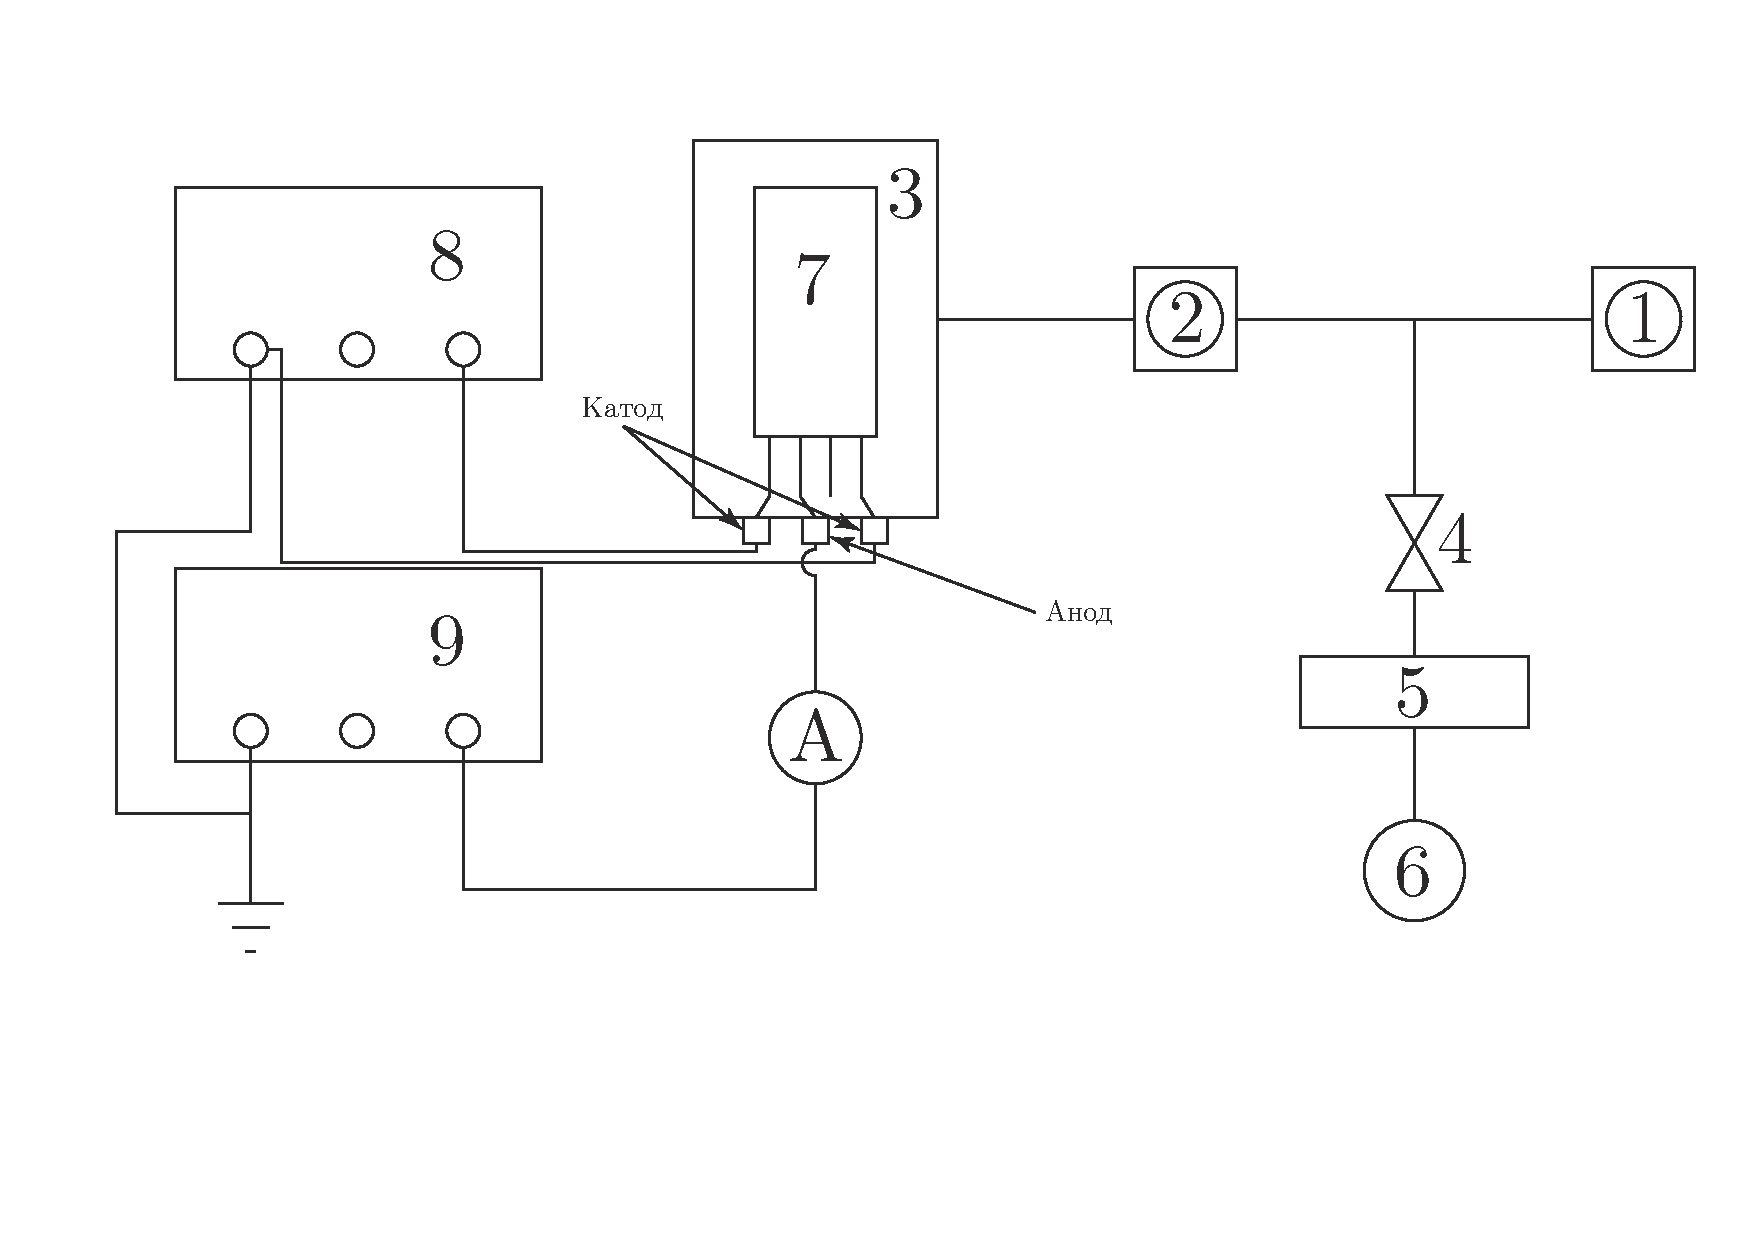
\includegraphics[scale=1.2]{scheme.pdf}
	\caption{Блок-схема установки по изучению рассеяния $\gamma$-квантов}
	\label{scheme}
\end{figure}
\par
Кванты, испытавшие комптоновское рассеяние в мишени, регистрируются сцинтилляционным счетчиком. Счетчик состоит из фотоэлектронного умножителя 3 (далее ФЭУ) и сцинтиллятора 4. Сцинтиллятором служит кристалл NaI(Tl) цилиндрической формы диаметром 40 мм и высотой 40 мм, его выходное окно находится в оптическом контакте с фотокатодом ФЭУ. Сигналы, возникающие на аноде ФЭУ, подаются на ЭВМ для амлитудного анализа. Кристалл и ФЭУ расположены в светонепроницаемом блоке, укрепленном на горизонтальной штанге. Штанга вместе с этим блоком может вращаться относительно мишени, угол поворота отситывается по лимбу 6.\par
Головная часть сцинтилляционного блока закрыта свинцовым коллиматором 5, который формирует входной пучок и защищает детектор от постороннего излучения. Основной вклад в это излучение вносят $\gamma$-кванты, проходящие из источника 1 через 6-сантиметровые стенки защитного контейнера. Этот фон особенно заметен при исследовании комптоновского рассеяния на большие углы ($\simeq 120^\circ$), когда расстояние между детектором и источником уменьшается.
\section{Ход работы}
\begin{enumerate}
	\item Включим все измерительные устройства и компьютер.
	\item Запустим программу и войдем в режим измерения спектра.
	\item Проверим функционировании установки в этом режиме при малом времени экспозиции (порядка 1 минуты):
	\begin{enumerate}
		\item снимем спектр при $\theta=0^\circ$;
		\item установим угол $\theta\simeq 30^\circ$ и снова снимем спектр, убедимся в том, что фотопик смещается влево, в сторону меньших энергий;
		\item определим положения фотопиков (номера канала) на экране дисплея.
	\end{enumerate}
	\item Устанавливая сцинтилляционный счетчик под разными углами $\theta$ к первоначальному направлению полета $\gamma$-квантов и вводя значения этих углов в ЭВМ, снимем амплитудные спектры и определим положение фотопиков для каждого значения угла $\theta$. Измерения проводим с шагом $10^\circ$ в диапазоне от $0^\circ$ до $120^\circ$. Результаты измерений занесем в таблицу \ref{expdata}.
	\begin{table}[!htb]
		\centering
		\caption{Измерения}
		\label{expdata}
		\begin{tabular}{|c|c|c|c|c|c|c|}
			\hline
			№ & Угол & Канал & Счет & Время & Частиц & I, [1/c]\\
			\hline
			1 & 0 & 965 & 72185 & 190 & 2454826 & 12920.1 \\
			2 & 0 & 941 & 76192 & 203 & 2616307 & 12888.2 \\
			3 & 10 & 971 & 68089 & 178 & 2952234 & 16585.6 \\
 			4 & 20 & 888 & 73827 & 362 & 824413 & 2277.4 \\
 			5 & 30 & 735 & 51589 & 326 & 291273 & 893.5 \\
 			6 & 40 & 679 & 52698 & 322 & 208925 & 648.8 \\
 			7 & 50 & 604 & 42443 & 307 & 160762 & 523.7 \\
 			8 & 60 & 522 & 41123 & 305 & 137531 & 450.9 \\
 			9 & 70 & 459 & 49867 & 401 & 160465 & 400.2 \\
 			10 & 80 & 411 & 41004 & 358 & 131360 & 366.9 \\
 			11 & 90 & 365 & 39560 & 375 & 129516 & 345.4 \\
 			12 & 100 & 332 & 31455 & 306 & 101375 & 331.3 \\
 			13 & 110 & 307 & 29843 & 309 & 100563 & 325.4 \\
 			14 & 120 & 302 & 33041 & 337 & 106722 & 316.7 \\
 			15 & 121 & 664 & 25445 & 197 & 99787 & 506.5 \\
 			16 & 122 & 835 & 47502 & 378 & 196851 & 520.8 \\
 			\hline
		\end{tabular}
	\end{table}
	\item Используя экспериментальные результаты, построим график (рис. \ref{fig:graph}), откладывая по оси абсцисс величину $1-\cos\theta$, а по оси ординат величину $1/N(\theta)$. Проведем через полученные точки наилучшую прямую.
	\begin{figure}[!htb]
		\includegraphics[width=\textwidth]{graph.pdf}
		\caption{График зависимости $\frac{1}{N}=f\left(1-\cos\theta\right)$}
		\label{fig:graph}
	\end{figure}
	\item Заменим в формуле \ref{eq2} энергию квантов испытавших комптоновское рассеяние на угол $\theta$, номером канала $N(\theta)$, соответствующего вершине фотопика при указанном угле $\theta$. Обозначая буквой $A$ неизвестный коэффициент пропорциональности между $\varepsilon(\theta)$ и $N(\theta)$, найдем:
	\begin{equation}
		\frac{1}{N(\theta)}-\frac{1}{N(0)}=A(1-\cos\theta).
		\label{eq:3}
	\end{equation}
	\par
	Согласно формуле (\ref{eq:3}) экспериментальные точки должны лежать на одной прямой. Пересечение этой прямой с осью ординат определяет наилучшее значение $N_{\text{наил}}(0)$. Это значение учитывает не только непосредственно измеренную величину $N(0)$, но и измерения сделанные под другими углами, а пересечение линии с прямой $\cos\theta=0$ позволяет найти наилучшее значение $N_{\text{наил}}(90)$. Таким образом можно найти энергию покоя частиц, на которых происходит комптоновское рассеяние. Снова обратимся к формуле (\ref{eq2}). Возвращаясь от переменной $\varepsilon$ к энергии $E$, мы получаем, что при $\theta=90^\circ$ формула (\ref{eq2}) принимает вид
	\begin{equation*}
		mc^2\left(\frac{1}{E(90)}-\frac{1}{E(0)}\right)=1,
	\end{equation*}
	или
	\begin{equation}
		mc^2=E(0)\frac{E(90)}{E(0)-E(90)}=E_\gamma\frac{N(90)}{N(0)-N(90)}.
		\label{eq:4}
	\end{equation}
	где $E(0)=E_\gamma$ -- энергия электронов, рассеянных вперед -- равна энергии $\gamma$-лучей, испускаемых источником ($^{137}$Cs).\par
	\item С помощью графика и формулы (\ref{eq:4}) определим энергию покоя частицы, на которой происходит комптоновское рассеяние первичных $\gamma$-квантов.
	\begin{equation*}
		E_r=\frac{N(90)}{N(0)-N(90)}=0.662\cdot\frac{373.23}{926.48-373.23}=0.447 \text{МэВ}.
	\end{equation*}
\end{enumerate}
\section{Вывод}
В ходе работы мы наблюдали рассеяние свободных гамма-квантов на свободных электронах графита. В ходе эксперимента выяснен интересный характер диаграммы направленности излучения источника $\gamma$-квантов: при больших углах обнаруживаются фоновые $\gamma$-кванты, проходящие через боковую стенку источника.  По результатам опыта была получена масса покоя электрона: $447\,\text{кэВ}$. Табличное значение $511\,\text{кэВ}$, а значит наш эксперимент находится в хорошем согласии с теорией.
\end{document}